\section{Introducción}

En esta práctica vamos a realizar el nodo 1 del bloque 2, pero esta vez las
conexiones entre los dispositivos será fijada de antemano en una PCB, a la cual
se soldarán posteriormente los distintos componentes discretos y conectores
necesarios. Además, no usaremos interruptores físicos para activar el relé,
sino que solo podrá ser manejado desde Domoticz.

Primero empezaremos creando el proyecto desde una de las plantillas estándar,
la correspondiente al Arduino Pro Mini.

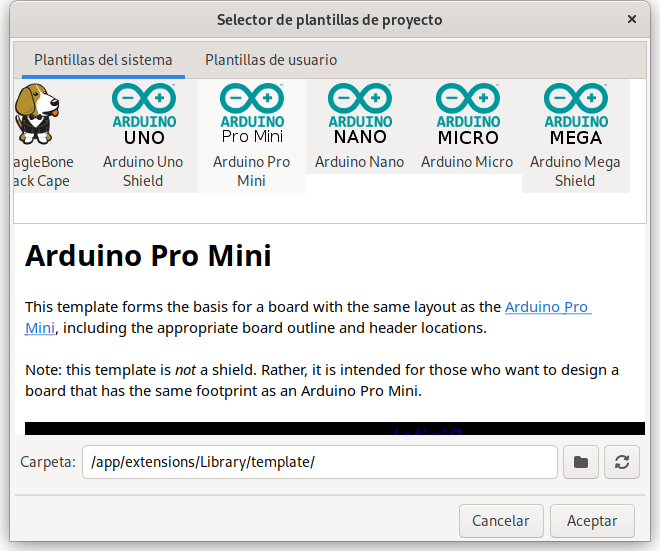
\includegraphics[width=\linewidth]{create-project-template.png}

Luego descargaremos los archivos de símbolo y huella del transistor
BC547C\footnote{\url{
    https://www.snapeda.com/parts/BC547C/ON/view-part/
}} y del relé G3MB-202P\footnote{\url{
    https://www.snapeda.com/parts/G3MB-202P/Omron\%20Automation/view-part/
}} y los descomprimiremos en la carpeta del proyecto de KiCad.

\section{Esquemática}

Abriremos la vista de esquemática haciendo doble click sobre el archivo de
extensión \verb|sch|. Una vez ahí, iremos a
\emph{Preferencias $\rightarrow$ Gestionar librerías de símbolos}, y añadiremos
las siguientes entradas en la pestaña
\emph{Librerías específicas del proyecto}:

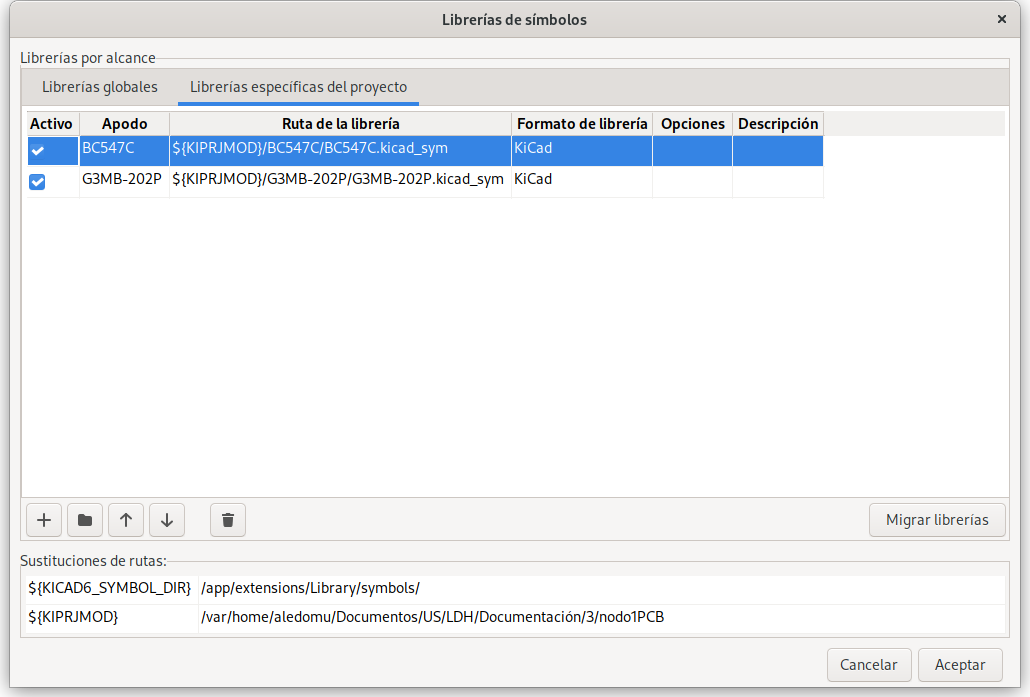
\includegraphics[width=\linewidth]{symbol-path.png}

Una vez importados los símbolos externos necesarios, formaremos la siguiente
esquemática del circuito:

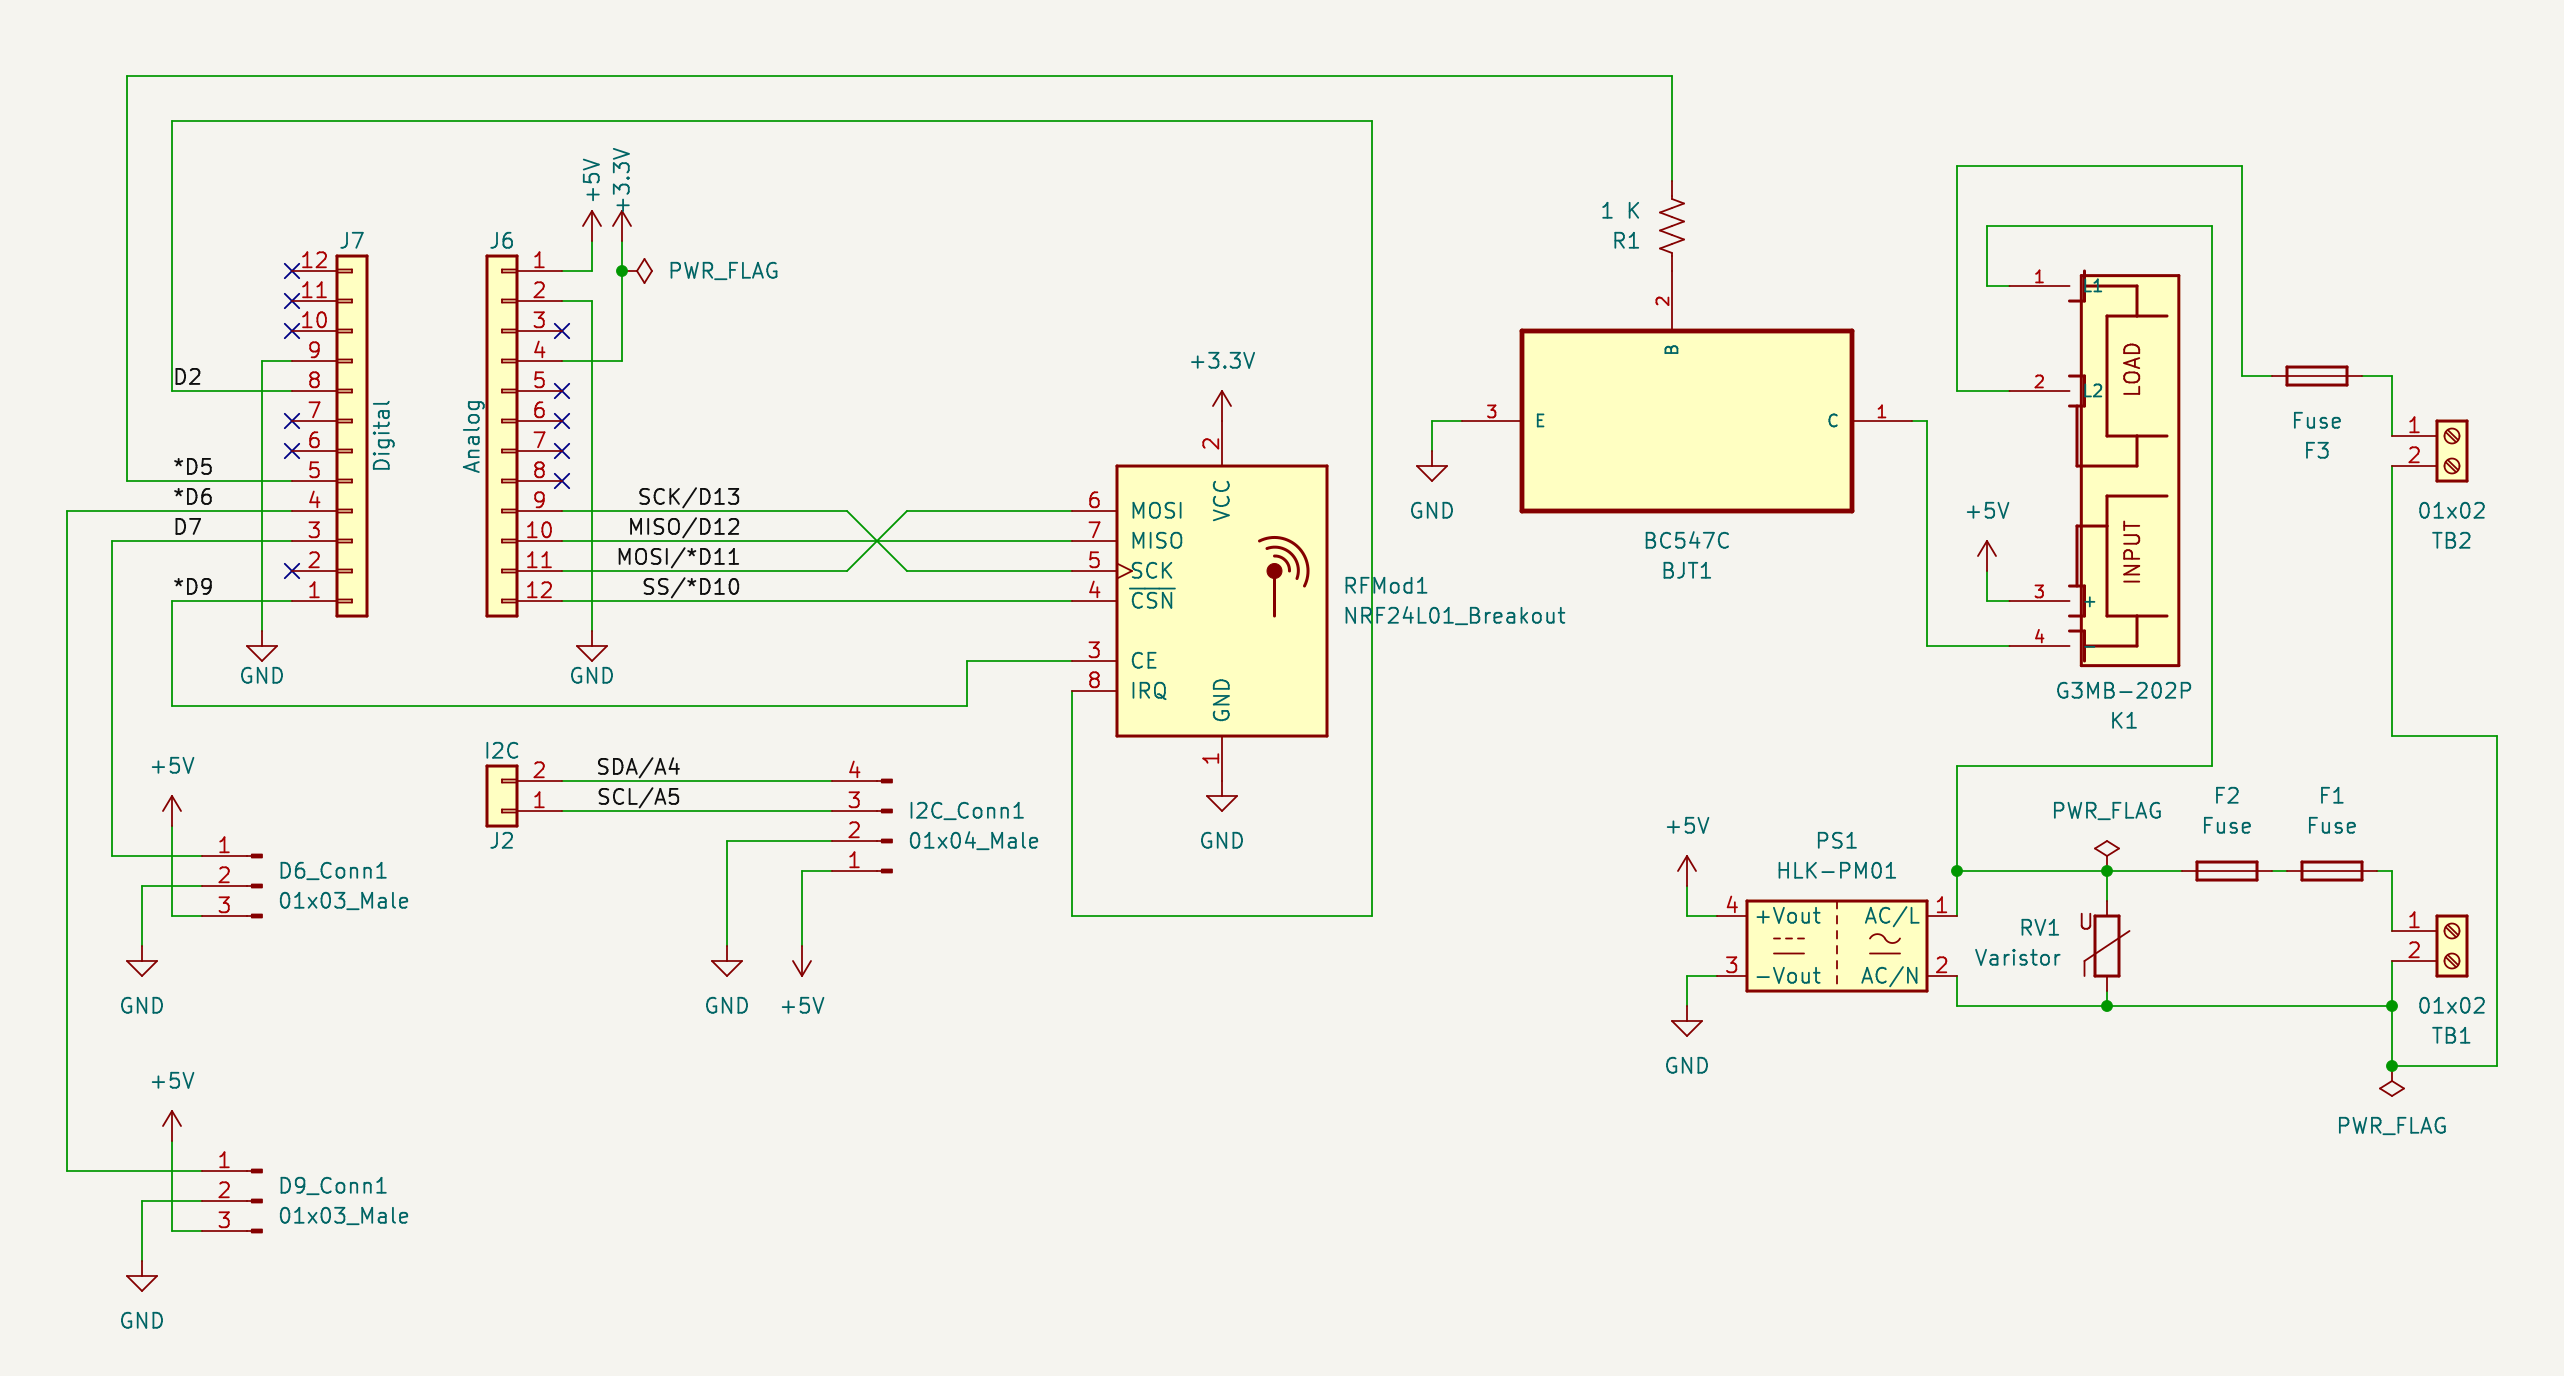
\includegraphics[width=\linewidth]{schematic-general.png}

Nótese que el pin correspondiente a la señal de interrupción del
radiotransmisor está conectado al pin 2 de la placa Arduino.

Finalmente, se deben rellenar los indicadores de referencia de los símbolos de
esquema y comprobar que se cumplen las reglas eléctricas sin un solo error.

\section{Asignación de huellas}

Antes de pasar al diseño de la distribución de los componentes en la PCB,
deberemos ajustar la relación entre componentes y huellas para mantener la
correlación entre la esquemática y el layout. Abriremos la herramienta para
asignar las huellas, en la que primero deberemos importar las huellas
necesarias yendo a
\emph{Preferencias $\rightarrow$ Gestionar librerías de huellas} y añadiendo
las siguientes entradas en la pestaña
\emph{Librerías específicas del proyecto}:

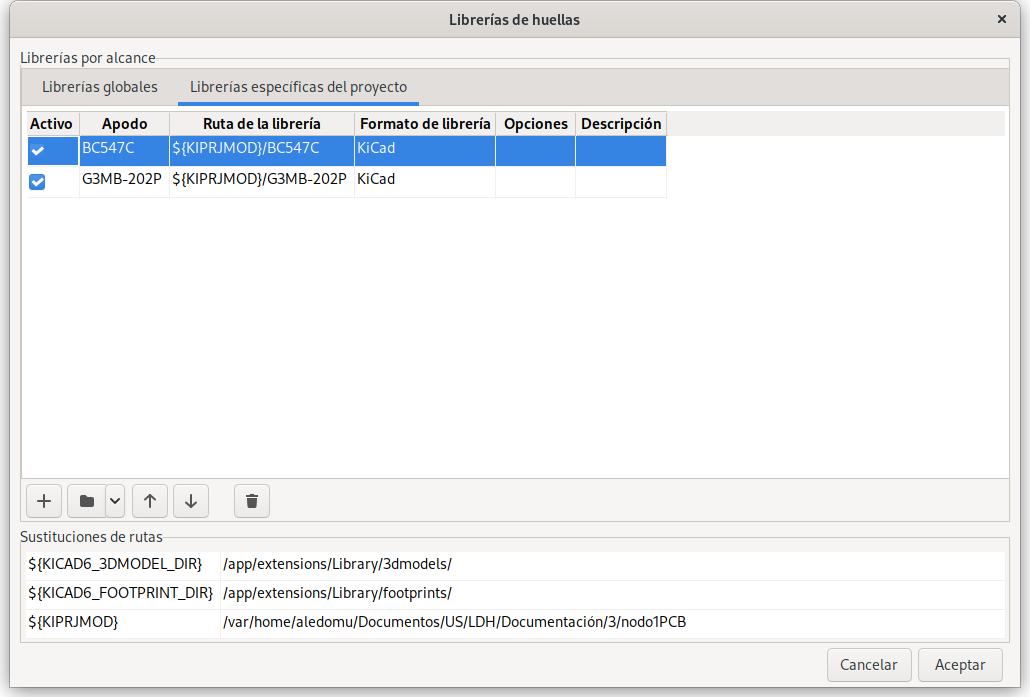
\includegraphics[width=\linewidth]{footprint-path.png}

Una vez importadas las huellas, la asignación que estableceremos es la
siguiente:

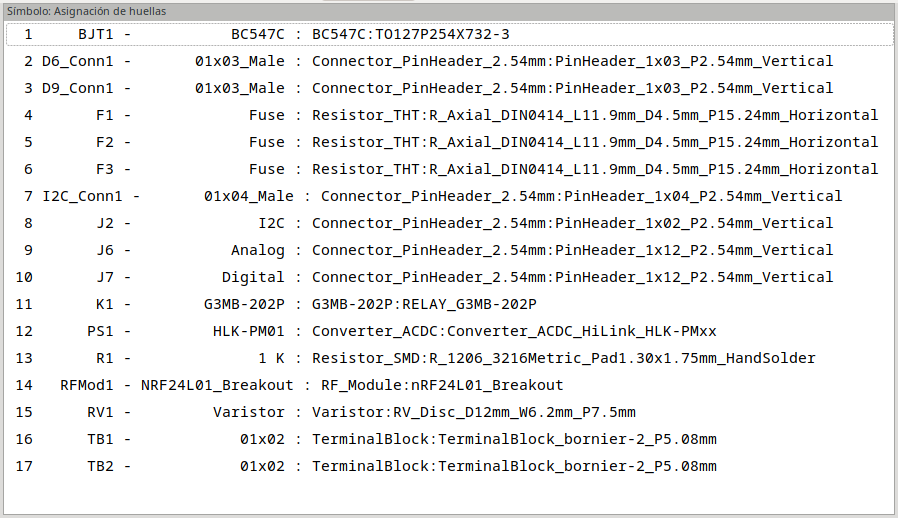
\includegraphics[width=\linewidth]{footprint-assignment.png}

La huella del transistor BJT que se usa es externa, importada anteriormente,
dado que la estándar genera un diseño cuyo resultado da lugar a una PCB en la
que la soldadura del componente es bastante más difícil porque los orificios
están más próximos entre sí.

Ahora sí, desde la vista de esquemática, abrimos la placa en el editor de
placas.

\section{Layout}

En esta fase del diseño de la PCB debemos distribuir espacialmente los
distintos elementos y sus interconexiones, que se realizarán en la capa de
cobre posterior (bottom). Además, como el único resistor que hay en el circuito
se monta de manera superficial (SMD), este hay que cambiarlo de lado en el menú
contextual.

En principio el límite de tamaño con el que contamos es de $10 \times 6$ cm,
pero si se ajusta como se indica en la imagen, se puede reducir a
$9 \times 6$ cm:

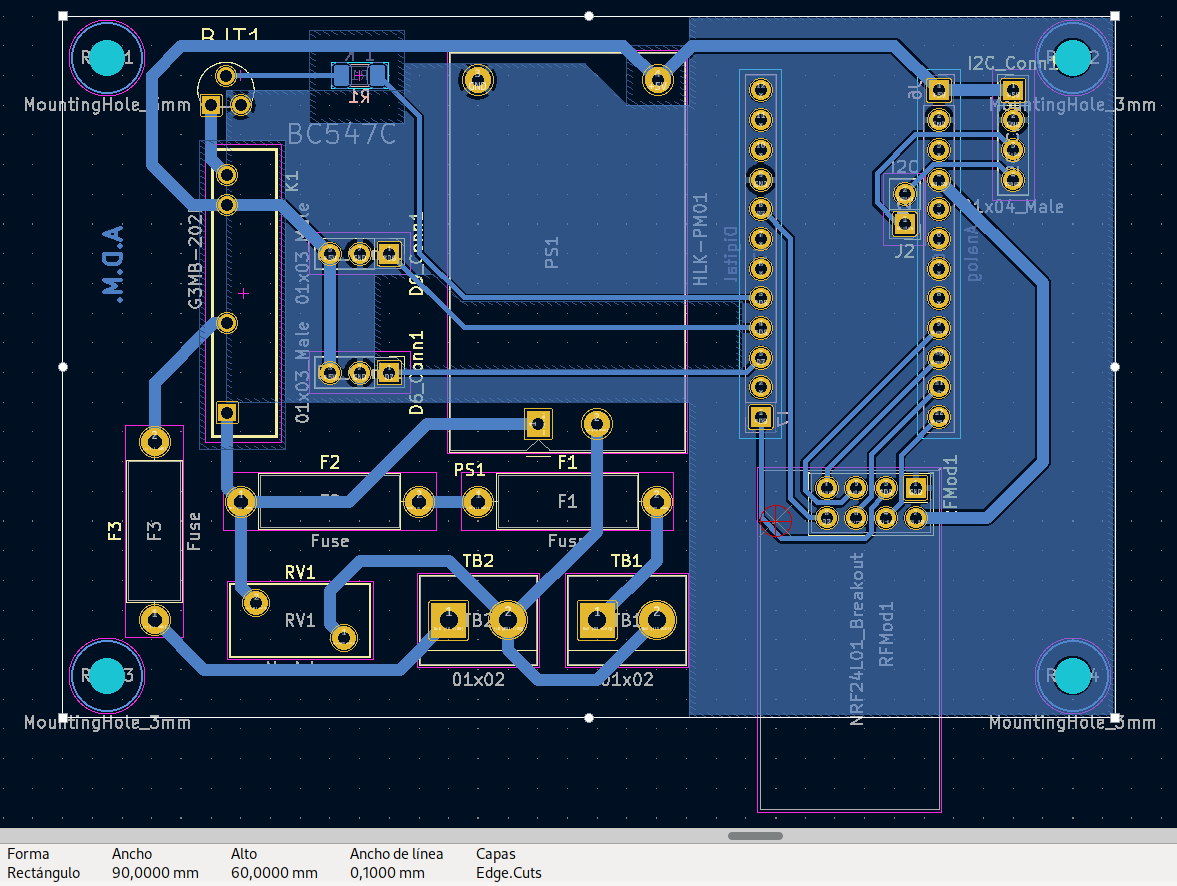
\includegraphics[width=\linewidth]{layout.png}

Las pistas que transmiten señales de alimentación deben tener un grosor de
1 mm, y las que transmiten señales digital deben ser de 0,406 mm. Este último
tamaño no existe de manera predefinida, por lo que se debe editar la lista de
tamaños predefinidos.

La conexión a tierra se establece mediante áreas de cobre que estarán unidasa a
los pads correspondientes a la conexión a tierra de la alimentación en
corriente continua.

Además hay que cambiar el tamaño de los pads del varistor para que el orificio
tenga un tamaño de 1 mm, y el pad en su conjunto de 2 mm. Para ello, hay que
seleccionar ambos e ir a sus propiedades en el menú contextual.

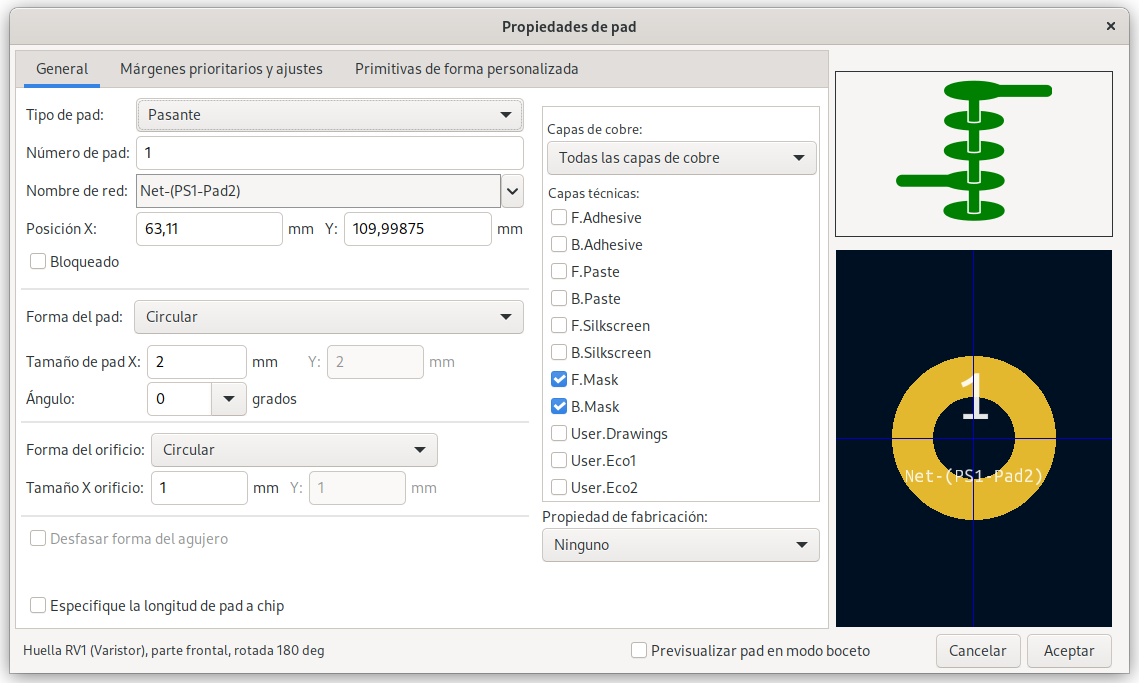
\includegraphics[width=\linewidth]{varistor-pad-hole-size.png}

\section{Trazado}

Una vez acabado el diseño, generaremos los archivos Gerber, necesarios para la
máquina que fabrica la PCB. Para ello iremos a
\emph{Archivo $\rightarrow$ Trazar} y especificaremos los siguientes
parámetros:

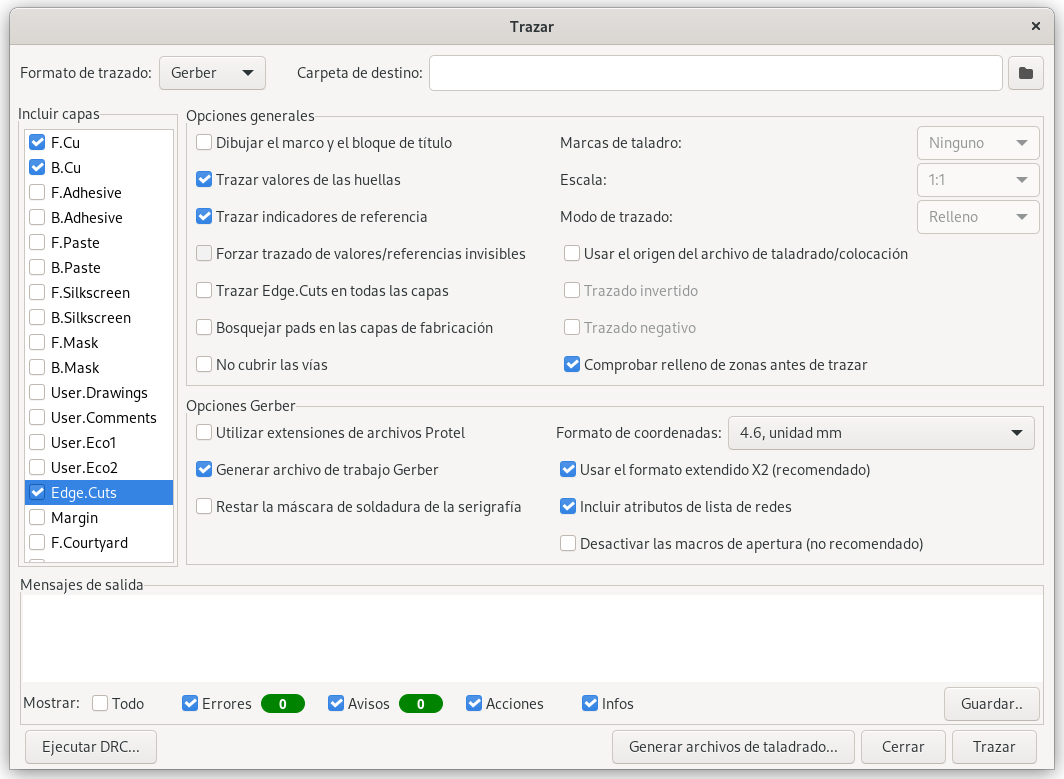
\includegraphics[width=\linewidth]{gerber-file-generation.png}

Primero le damos a \emph{Generar archivos de taladrado}. Nos saldrá otra
ventana, en la que pondremos los siguientes ajustes:

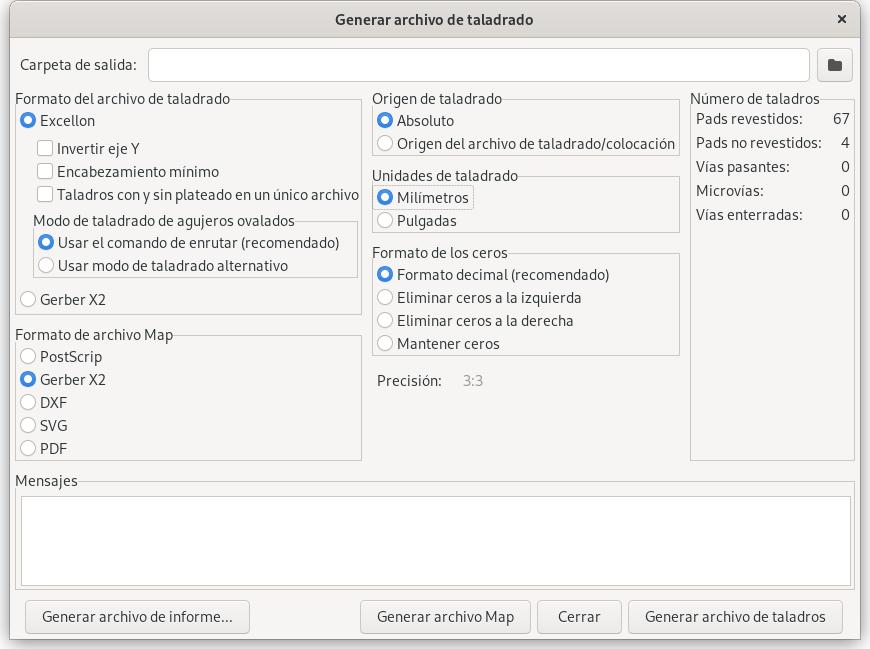
\includegraphics[width=\linewidth]{gerber-drilling-file-generation.png}

Es importante indicar que las unidades de taladrado sean en milímetros para que
los archivos resultantes sean utilizables por la máquina del departamento de la
asignatura, y así poder tener la placa PCB con las especificaciones correctas.

Pulsaremos primero \emph{Generar archivo Map} y luego
\emph{Generar archivo de taladros}. Finalmente, cerramos esta ventana y nos
aparecerá de nuevo la primera, en la que pulsaremos \emph{Trazar}. Deberíamos
tener los archivos correspondientes en la carpeta \verb|output| dentro del
directorio del proyecto.

\section{Análisis del diseño en webs de encargo a fabricación}

Los diseños de PCBs pueden subirse a ciertas páginas web para que expongan
cierta información adicional de los mismos. Para ilustrarlo, usaremos la
utilidad de Eurocircuits\footnote{\url{https://www.eurocircuits.com/}}. Aunque
existen otras, Eurocircuits ofrece un grado de detalle incomparablemente mayor,
por lo que nos limitaremos a esta web.

Eurocircuits permite realizar el pedido inmediatamente una vez hechos los
ajustes pertinentes. Para ello, desde la misma dirección principal, cargaremos
el archivo de layout de KiCad (extensión \verb|pcb|) directamente, dado que
también lo admite además de los gerbers. Podría cargarse también el BOM (Bill
Of Materials), pero no es nuestro objetivo realizar un presupuesto de
ensamblaje completo desde fábrica, así que lo omitiremos.

Para tener un análisis completo, debemos tener una cuenta con la sesión
iniciada y, tras cargar el archivo, añadir la placa al
\emph{carro de la compra} para realizar el análisis completo, el cual tardará
unos minutos. Luego pulsamos en \emph{PCB Visualizer} y veremos los siguientes
datos:

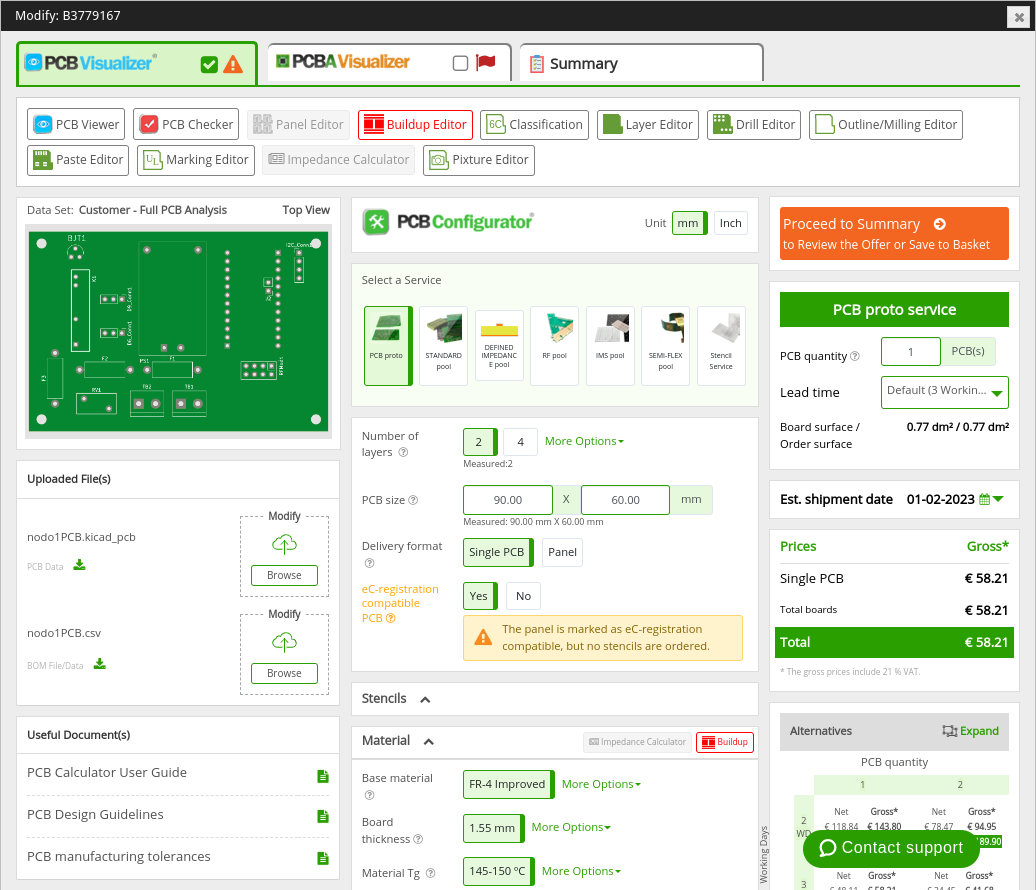
\includegraphics[width=\linewidth]{eurocircuits-pcb-viewer-1.png}

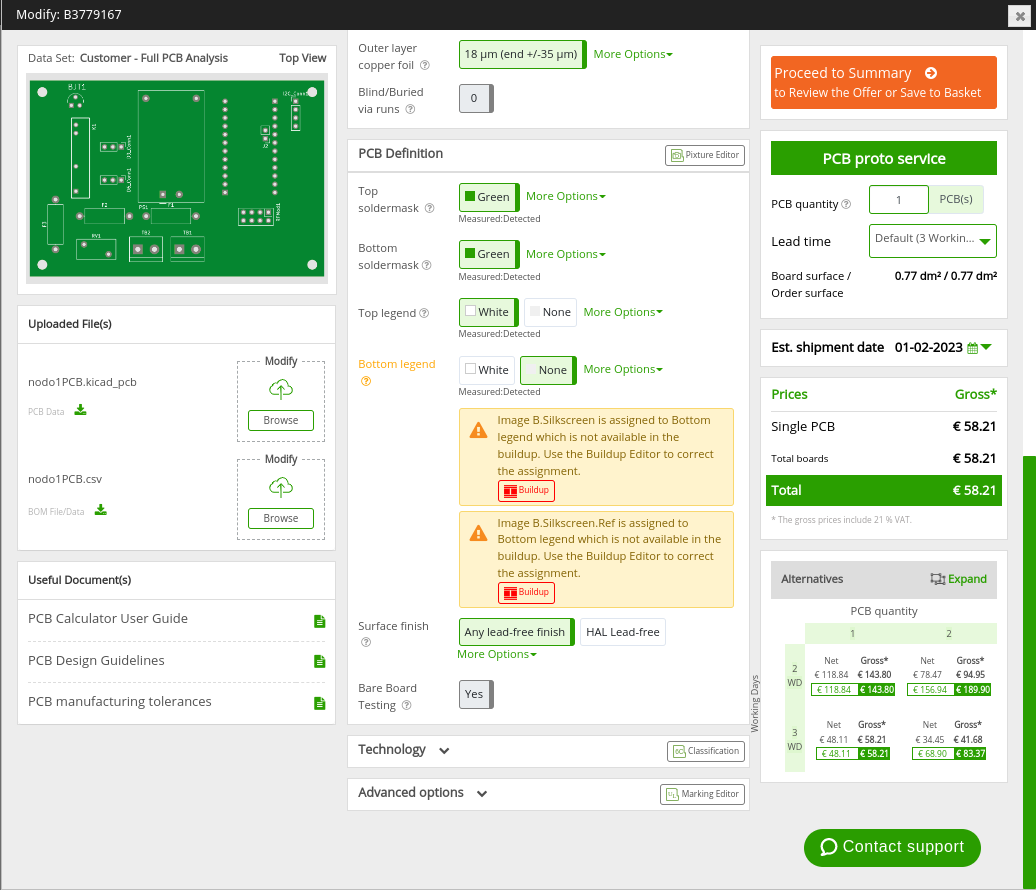
\includegraphics[width=\linewidth]{eurocircuits-pcb-viewer-2.png}

Podemos ver que detecta que la placa tiene dos capas y que su tamaño es de
$9 \times 6$ cm. Además, hay tres advertencias, la primera tiene que ver con
las zonas SMD y las otras dos con la asignación de capas de la leyenda impresa.
La propia herramienta guía de manera relativamente sencilla qué correcciones
hacer.

En base al diseño, también se eligen las opciones más adecuadas. Además, se
pueden realizar ciertas modificaciones. También se puede generar un informe con
la información más importante de la lista de pedidos.

Para usar otras herramientas, hay que generar los archivos gerber de todas las
capas y comprimirlos en un archivo zip. Para ello, hay que repetir los pasos de
la sección de trazado y además seleccionar todas las capas.

\section{Ensamblaje}

El proceso estándar de soldado se realiza poniendo en contacto la punta del
soldador con el terminal del dispositivo colocado en el orificio
correspondiente durante no más de siete segundos a 350 ºC, durante los cuales
se debe también aproximar el hilo de estaño para fundirlo entre la superficie
de cobre, sin exceder los límites de la pista, y el conector terminal.
Previamente hay que colocar fundente en el área, pudiendo ser incluso líquido
depositado con un pincel. La ventilación del lugar debe ser adecuada y hay que
encender un extractor a poca distancia de donde se realice la operación para
evitar inhalar los vapores del fundente y la propia fundición.

En caso de que una soldadura se salga del límite de pista ocasionando una
conexión no deseada, se puede sacar interponiendo una malla de desoldadura
entre la zona y la punta si el exceso es pequeño, disparando una bomba de
desoldar mecánica mientras se refunde el estaño o usando una estación
desoldadora.

Uno de los fusibles es térmico para proteger el circuito de
sobrecalentamientos. El problema de este componente es que la temperatura del
proceso de soldadura puede romperlo, haciendo que deje de conducir. Para
mitigar este riesgo hay que dejar todo el largo a los terminales del fusible,
sin que sobresalga por debajo, y realizar una soldadura a menor temperatura con
muy buen apoyo, con la punta del soldador pegada no más de cuatro segundos.

Los fusibles restantes son de intensidad. Tanto ellos como el varistor pueden
introducirse recortando la longitud de sus terminales al máximo.

Otra particularidad reside en la soldadura del resistor, que se realiza en
superficie. Para que sea exitosa, en lugar de usar un hilo de estaño, se usa
una pasta de estaño entre cada zona de cobre y cada conector del resistor, y se
acerca la punta del soldador caliente directamente, fundiendo la pasta y
pegando el componente a las dos zonas de cobre por separado.

\section{Testado}

Al mismo tiempo que se va realizando el ensamblaje, hay que ir comprobando con
un multímetro que hay conductividad \emph{solo} entre las soldaduras
requeridas. Es imperativo evitar cualquier cortocircuito con masa puesto que
aquí estamos trabajando con tensiones de 220 V. Si hay conductividad donde no
debe haberla, eso significa que alguna soldadura ha excedido los límites de la
pista. Si no hay conductividad donde sí debiera haberla, entonces la soldadura
está demasiado débil y se tiene que terminar.

\section{Programación del Arduino}

El microcontrolador lo cargaremos con el siguiente programa:

\lstinputlisting[language=C++, caption=nodo1PCB.ino]{3/nodo1PCB/nodo1PCB.ino}

Aquí estamos reutilizando la configuración de autenticación y/o encriptado que
haya sido usada en el bloque 2, junto con la del gateway en la Raspberry Pi.

\section{Resultado}

Tras soldar todos los componentes, la PCB debería quedar así:

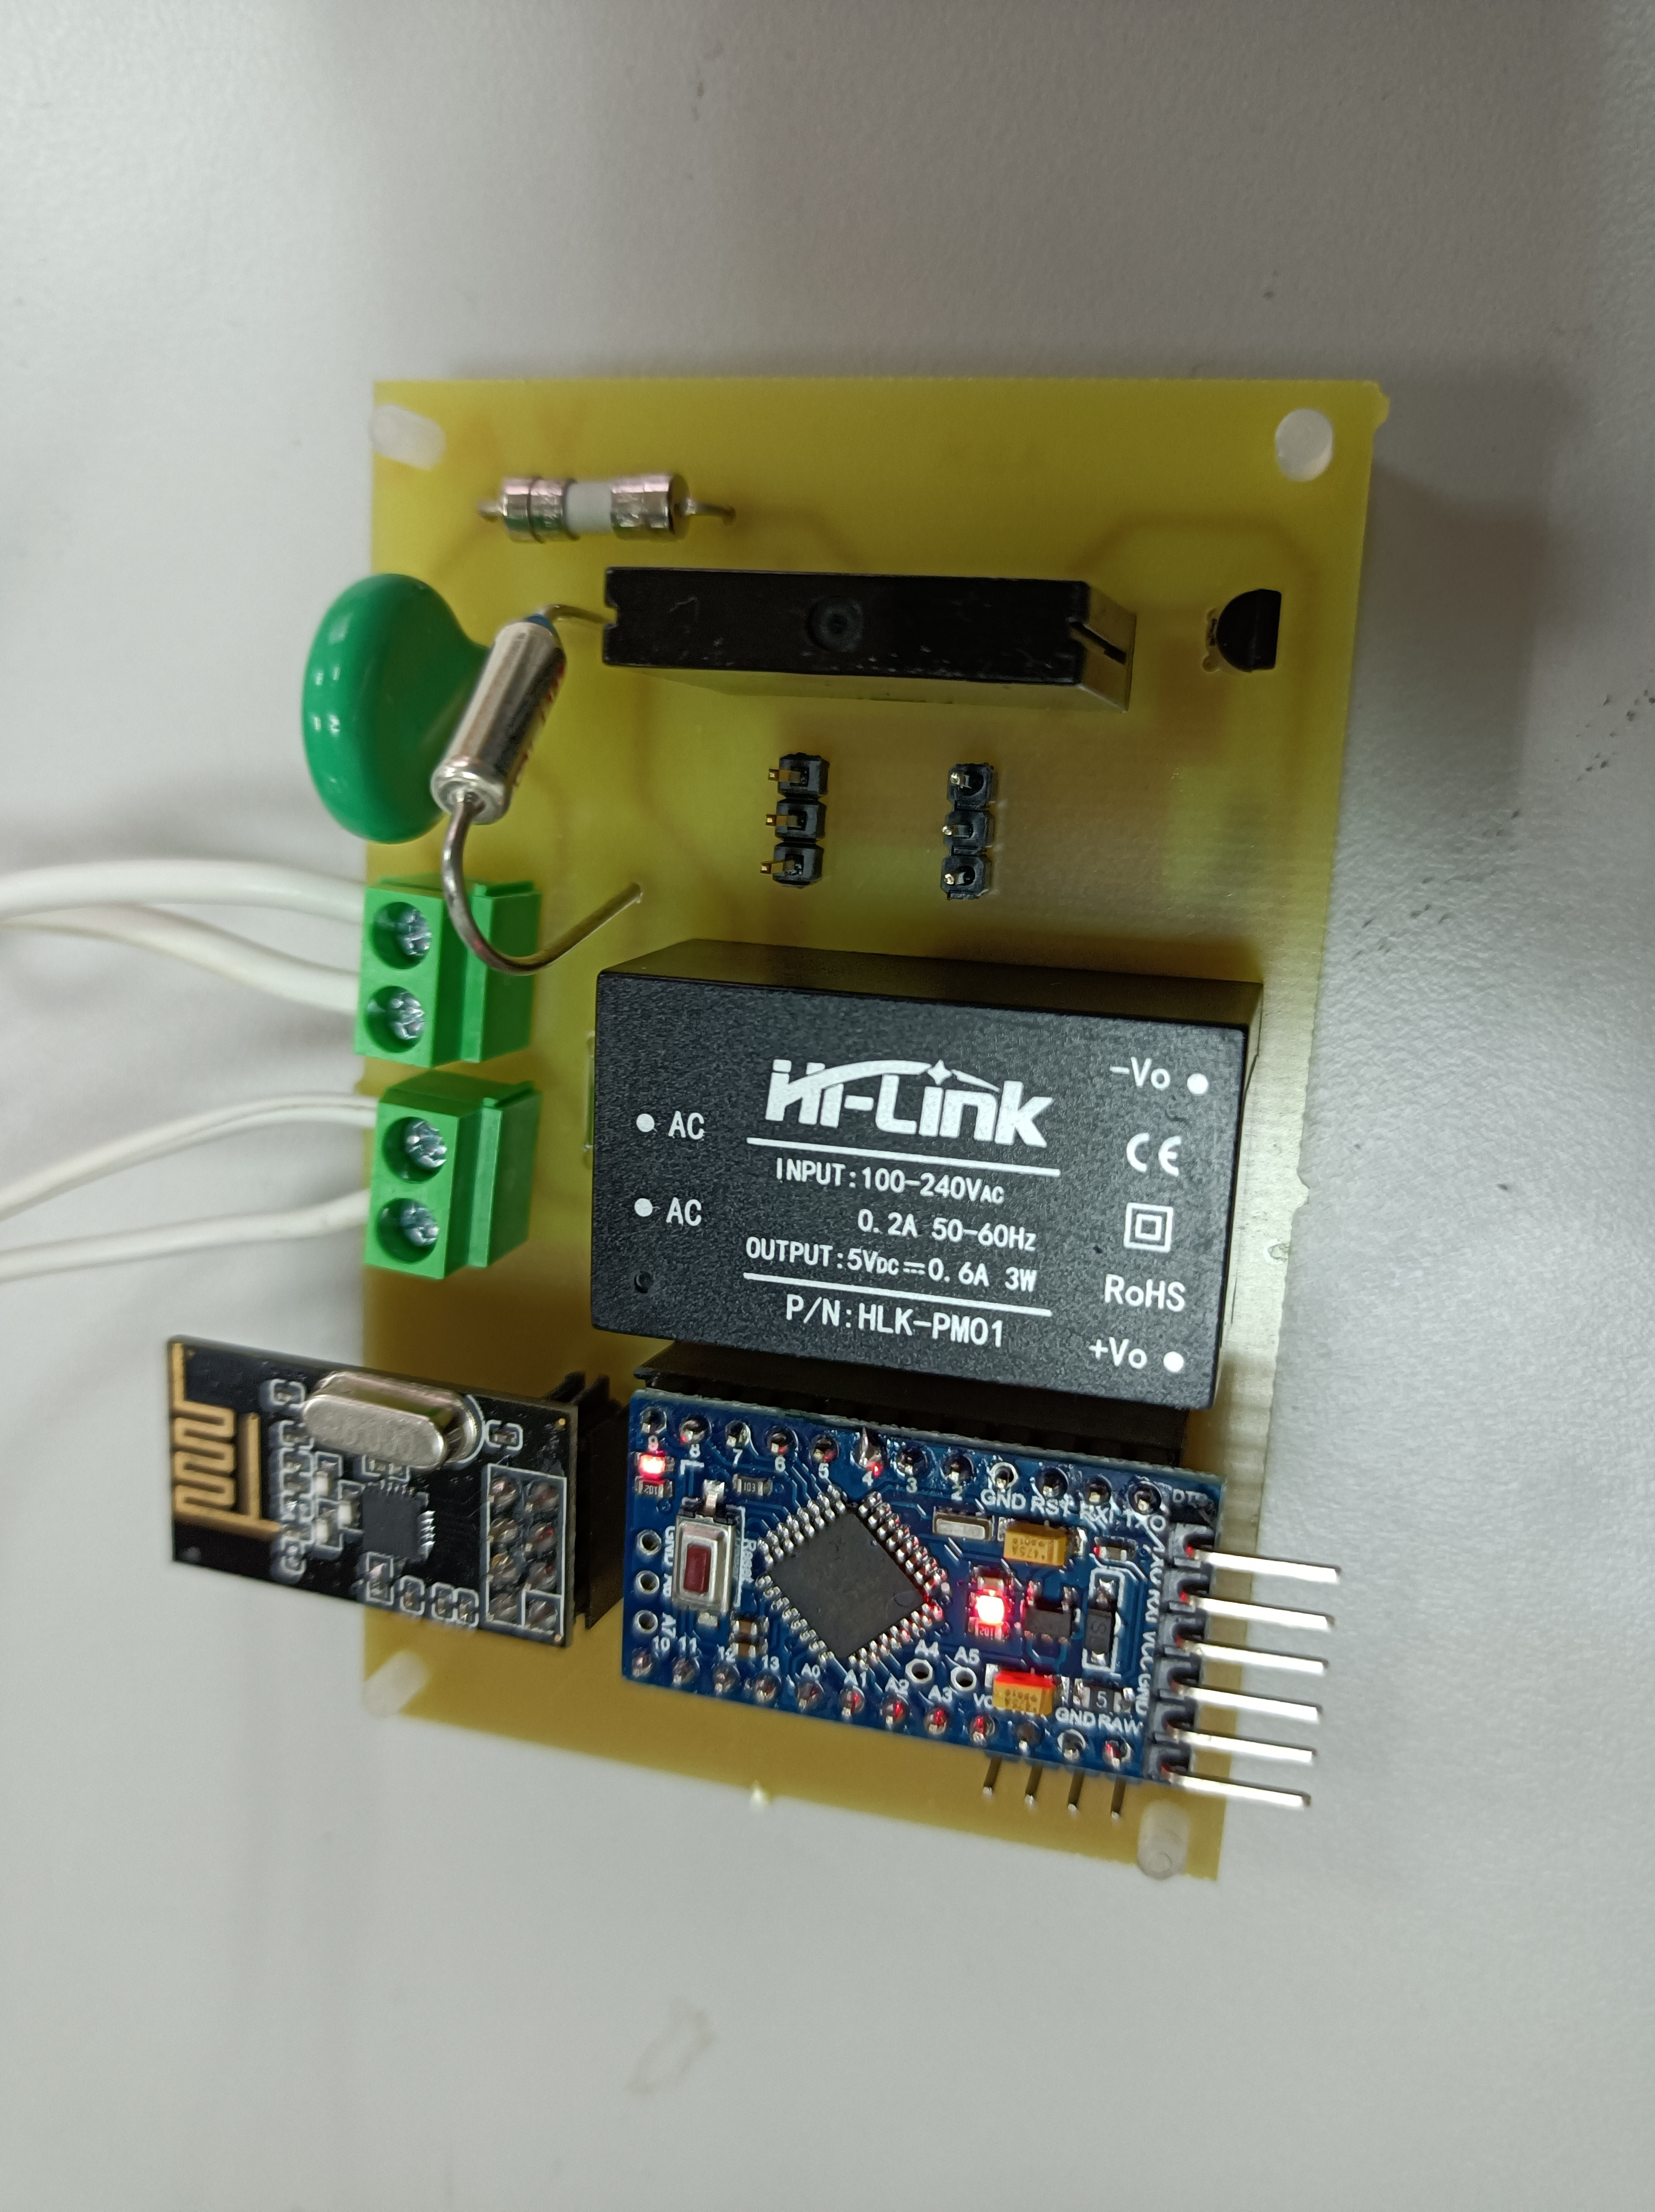
\includegraphics[width=\linewidth]{pcb-front.jpg}

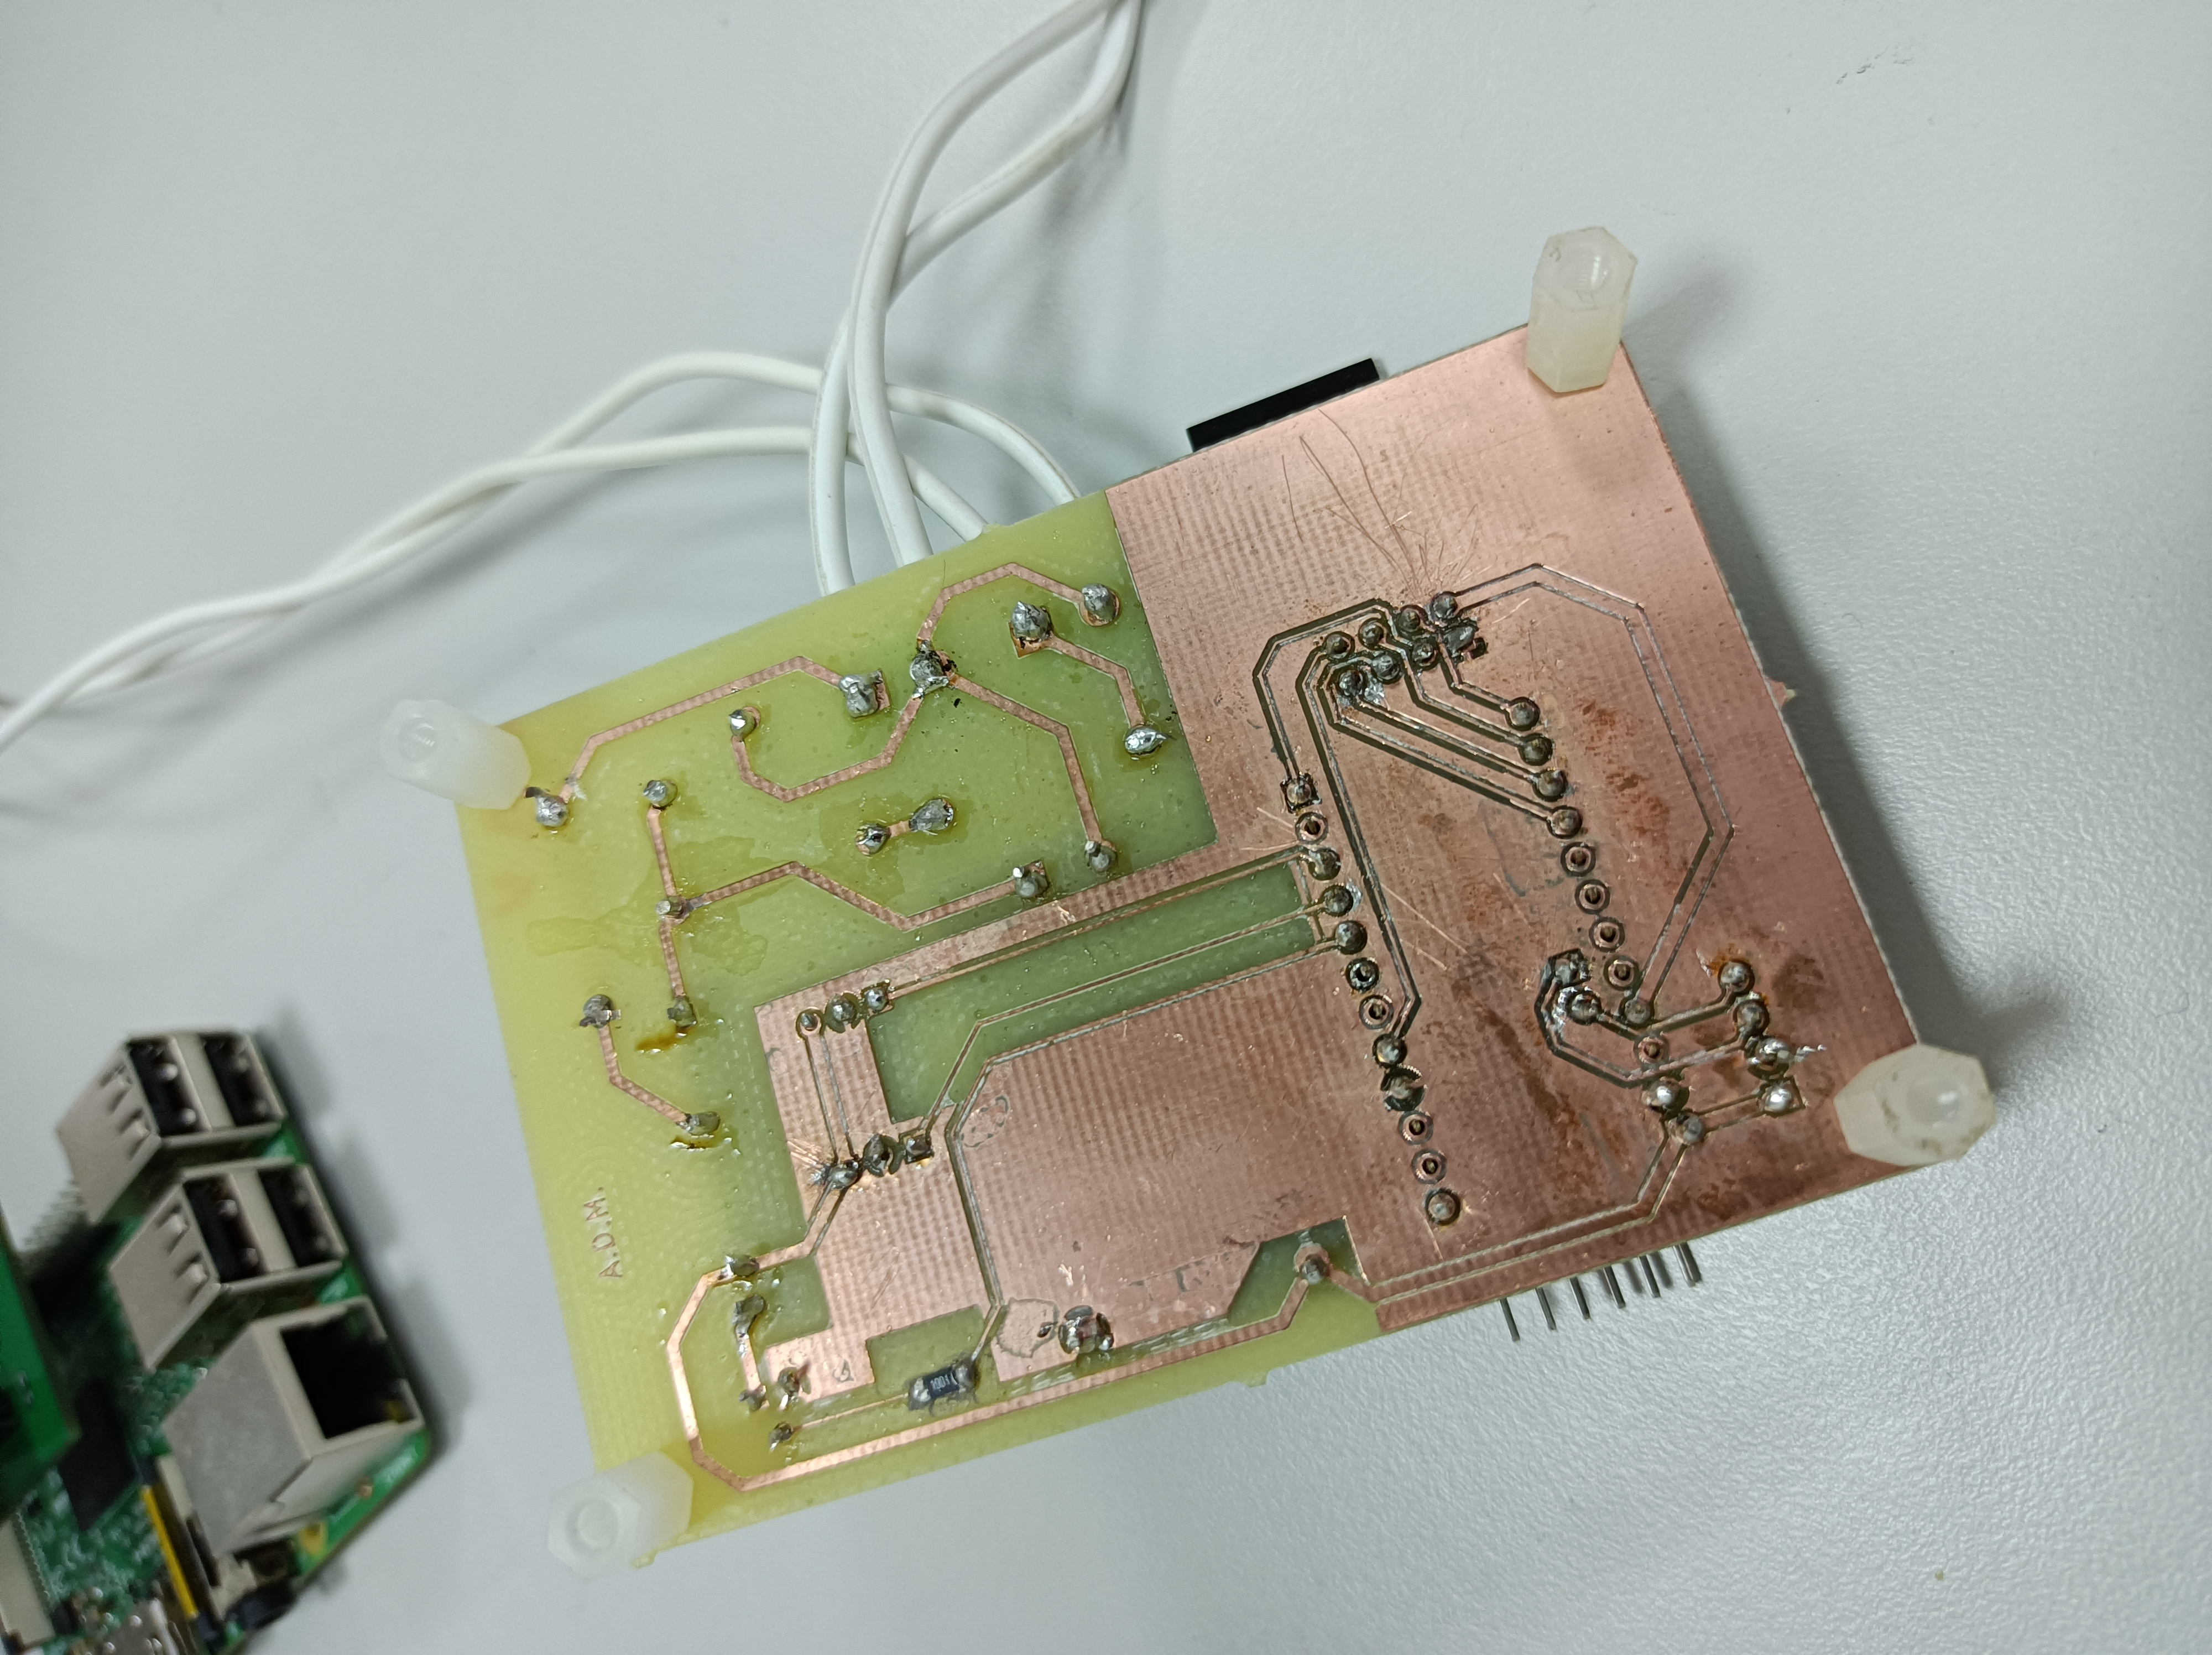
\includegraphics[width=\linewidth]{pcb-back.jpg}

Para ponerla a funcionar, hay que conectar uno de los terminales verdes a la
red doméstica y el otro a la luz o cualquier dispositivo preparado para
recibir 220 V de corriente alterna y no más de 2 A de intensidad. Con una luz
de tubo fluorescente encendida desde Domoticz queda así:

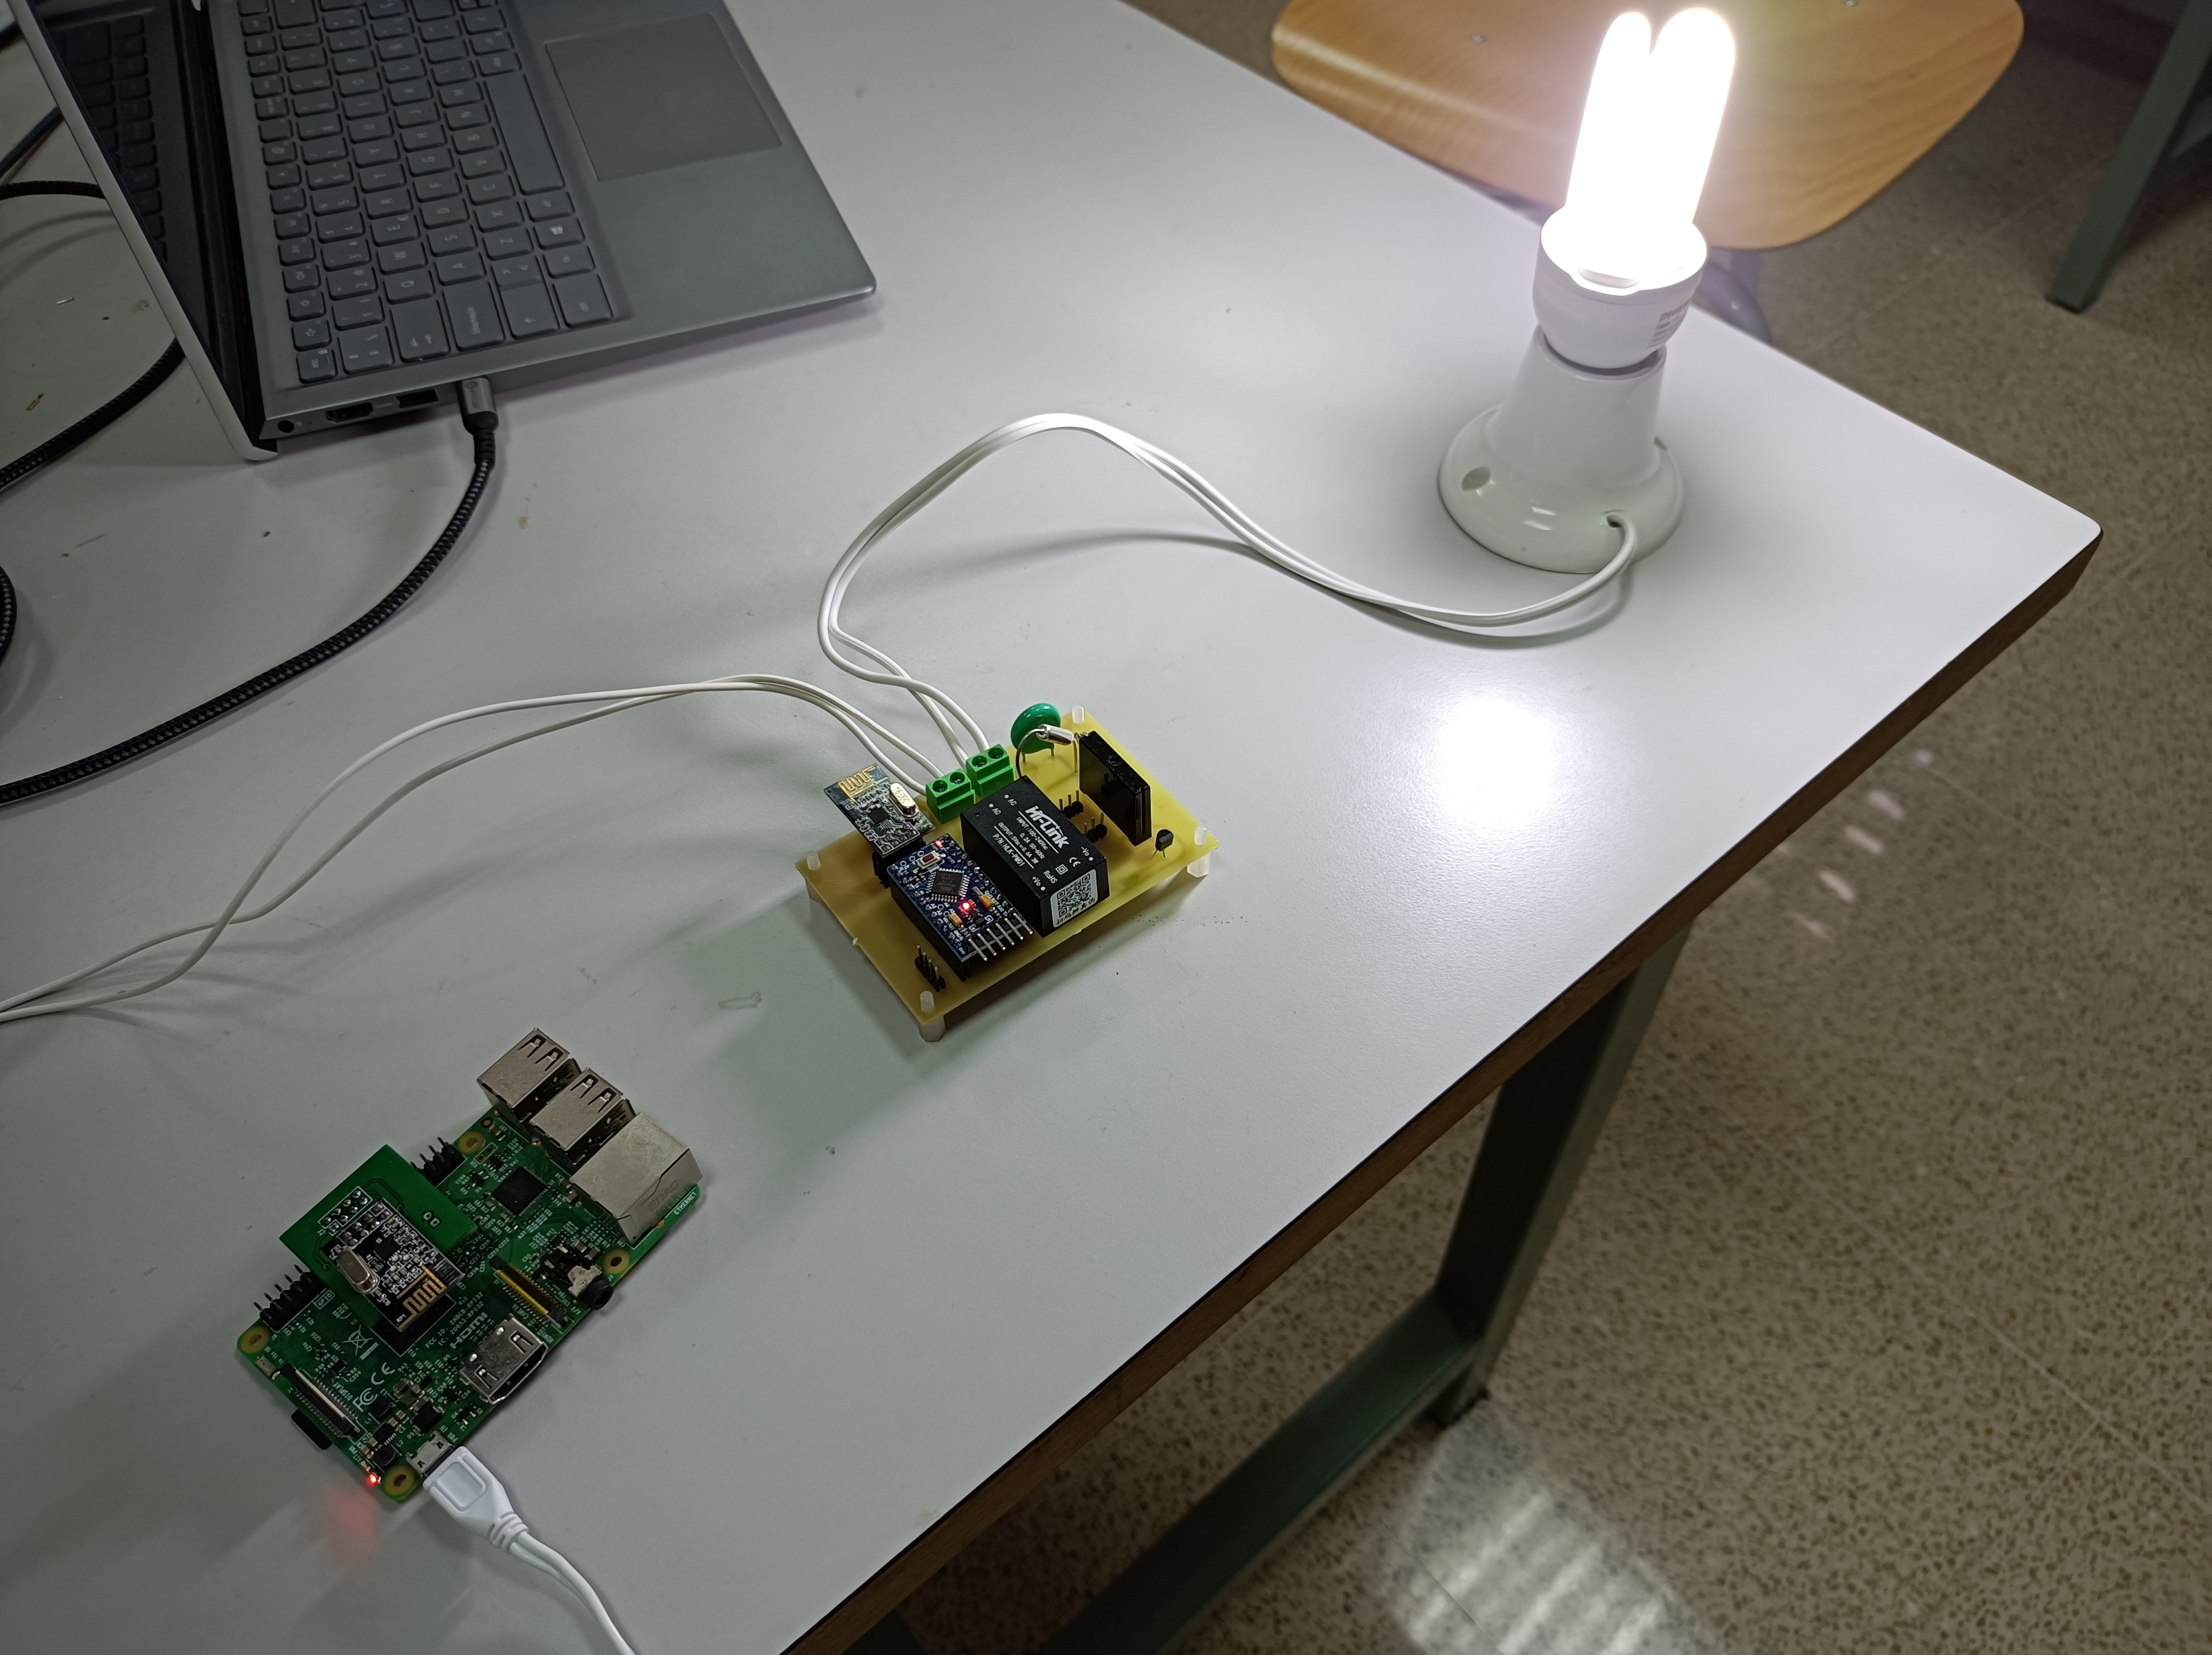
\includegraphics[width=\linewidth]{pcb-light-on.jpg}